%; whizzy document
% latex beamer presentation.
% platex, latex-beamer でコンパイルすることを想定。 


%     Tokyo Debian Meeting resources
%     Copyright (C) 2006 Junichi Uekawa

%     This program is free software; you can redistribute it and/or modify
%     it under the terms of the GNU General Public License as published by
%     the Free Software Foundation; either version 2 of the License, or
%     (at your option) any later version.

%     This program is distributed in the hope that it will be useful,
%     but WITHOUT ANY WARRANTY; without even the implied warranty of
%     MERCHANTABILITY or FITNESS FOR A PARTICULAR PURPOSE.  See the
%     GNU General Public License for more details.

%     You should have received a copy of the GNU General Public License
%     along with this program; if not, write to the Free Software
%     Foundation, Inc., 51 Franklin St, Fifth Floor, Boston, MA  02110-1301 USA


\documentclass[cjk,dvipdfmx]{beamer}
\usetheme{Warsaw}
%  preview (shell-command (concat "xpdf " (replace-regexp-in-string "tex$" "pdf"(buffer-file-name)) "&"))
%  presentation (shell-command (concat "xpdf -fullscreen " (replace-regexp-in-string "tex$" "pdf"(buffer-file-name)) "&"))

%http://www.naney.org/diki/dk/hyperref.html
%日本語EUC系環境の時
\AtBeginDvi{\special{pdf:tounicode EUC-UCS2}}
%シフトJIS系環境の時
%\AtBeginDvi{\special{pdf:tounicode 90ms-RKSJ-UCS2}}

\title[Debian 勉強会]{始動:Debian Multimedia Project}
\subtitle{2006年2月18日}
\author{上川}
\date{2006年2月18日}

\begin{document}

\frame{\titlepage{}}
 
 \section{Debian Multimedia}
 \subsection{まず、最初に}
 \begin{frame}
  \frametitle{DAWの定義}
   DAW: Digital Audio Workstation

   音楽録音編集に利用するワークス
	 テーション。一般家庭の常識からは考えられないようなメモリ容量(最
	 大まで積むのが基本)、静音性、ディスク速度、オーディオIOが期待さ
	 れる。無駄に10トラックから24トラック程度のオーディオ同時入出力
	 を備え、一般家庭に潜んでいる宅録を嗜好する方々が別用途で確保し
	 た予算を流用して資産を浪費するためのもの。
 \end{frame}
 
 \begin{frame}
  \frametitle{DAWの定義}
  DAW: Debian Audio Workstation

  
	 特に理由もなくDebianを使って、オーディオトラックを大量に利用し、
	 レコーディングやマスタリングをしてみようとすること。
	 2006年初旬までは苦難の道として知られていた。
	 Linuxカーネルのリアルタイム応答性などの改善により、
	 口コミで評判がひろまり
	 2007年中旬ころから大ブレークするかもしれない予定。
 \end{frame}


\begin{frame}
\frametitle{世界情勢}
 \begin{itemize}
  \item AGNULA/DeMuDi:
	EUの予算をとりつけて連合予算のもとで過去3年ほど開発が続けられて
	いたDebianベースのマルチメディアオーディオディストリビューション。
	このたびプロジェクト終了
  \item linux-audio-dev: 
	Linux の上で動くオーディオアプリの開発を調整するためのメーリング
	リスト。
	ladspa や jack が生まれた。すごい流量で、新しいソフトウェアがで
	きましたという発表メールの勢いも凄い。
  \item Debian-multimedia:
	ladspa や jack が複数のパッケージ間での調整が必要となることから、
	ブラジルにてマルチメディアミーティングをした。
	それと前後してできたメーリングリスト。主要なDebian開発者がDeMuDi
	で忙しかったことなどから結局3年くらい放置。
 \end{itemize}
\end{frame}


\begin{frame}
\frametitle{DAWの要素}
 \begin{itemize}
  \item オーディオ入出力
  \item MIDI
  \item ソフトウェアエフェクト
  \item ソフトウェアシンセサイザー
  \item オーディオ/MIDI シーケンサー
 \end{itemize}
\end{frame}

\begin{frame}
\frametitle{Linuxではどうなっているか}
 \begin{itemize}
  \item オーディオ入出力: ALSA audio, jack
  \item MIDI: ALSA MIDI
  \item ソフトウェアエフェクト: LADSPA
  \item ソフトウェアシンセサイザー: ALSA MIDIで駆動、jackで出力
  \item オーディオ/MIDI シーケンサー: audacity, muse, ardour, rosegarden
	など
 \end{itemize}
 オーディオ入出力制御のJackとMIDI入出力のALSA(MIDI)を駆使して操作することになる。
\end{frame}

 \subsection{どんなアプリケーションがあるのか}
\begin{frame}
 \frametitle{キーボードを仮想鍵盤として活用}
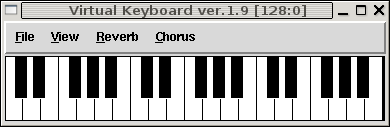
\includegraphics[width=10cm]{image200602/vkeybd.png}\\
 vkeybdは、とりあえず試すのに便利
\end{frame}

\begin{frame}
 \frametitle{qjackctl: 接続を制御}
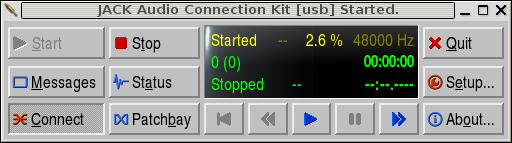
\includegraphics[width=10cm]{image200602/qjackctl-1.png}\\
jackdの起動や接続を制御する
\end{frame}

\begin{frame}
 \frametitle{qjackctl MIDI接続の制御}
 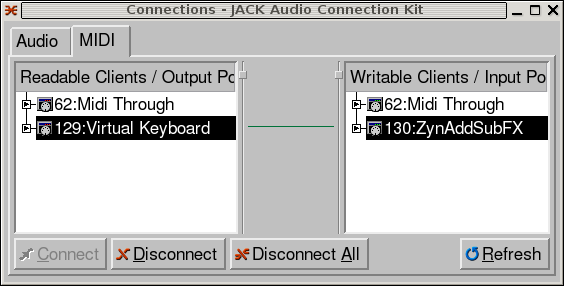
\includegraphics[width=10cm]{image200602/qjackctl-midi.png}\\
 MIDIでどう接続するのかを制御できる。
\end{frame}

\begin{frame}
 \frametitle{qjackctl}
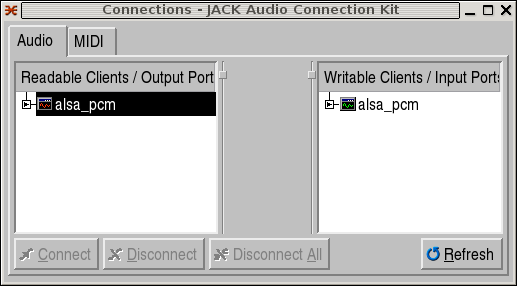
\includegraphics[width=10cm]{image200602/qjackctl-2.png}\\
 Jackでどう接続するのかを制御できる。
\end{frame}

\begin{frame}
 \frametitle{LADSPAエフェクトをかける}
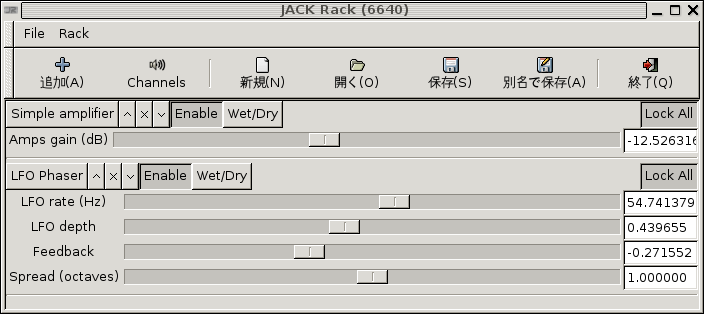
\includegraphics[width=10cm]{image200602/jack-rack.png}\\
Jack入力から取得した音をLADSPAのエフェクトをかけて、出力へ。\\
現状 300 以上のプラグインがあるみたい。
\end{frame}

\begin{frame}
 \frametitle{zynaddsubfx}
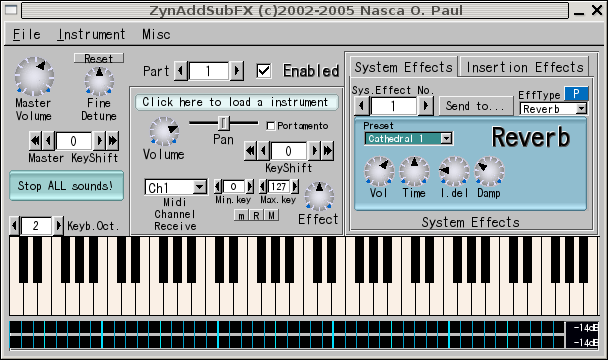
\includegraphics[width=10cm]{image200602/zynaddsubfx.png}
\end{frame}

\begin{frame}
 \frametitle{hydrogen}
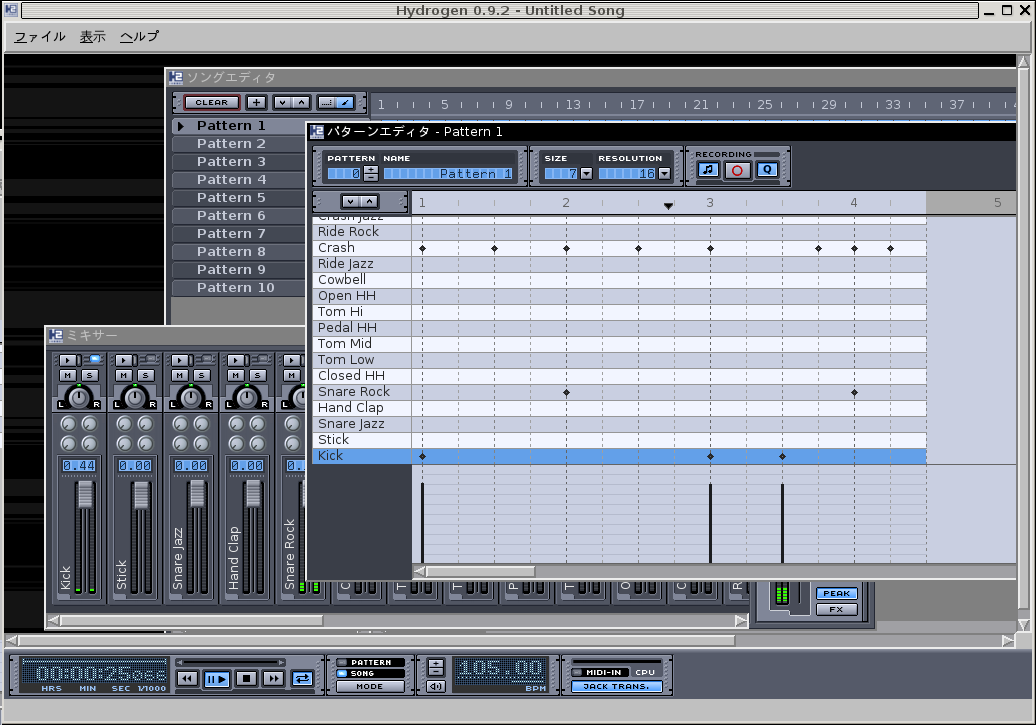
\includegraphics[width=10cm]{image200602/hydrogen.png}
\end{frame}

\begin{frame}
 \frametitle{rosegarden4}
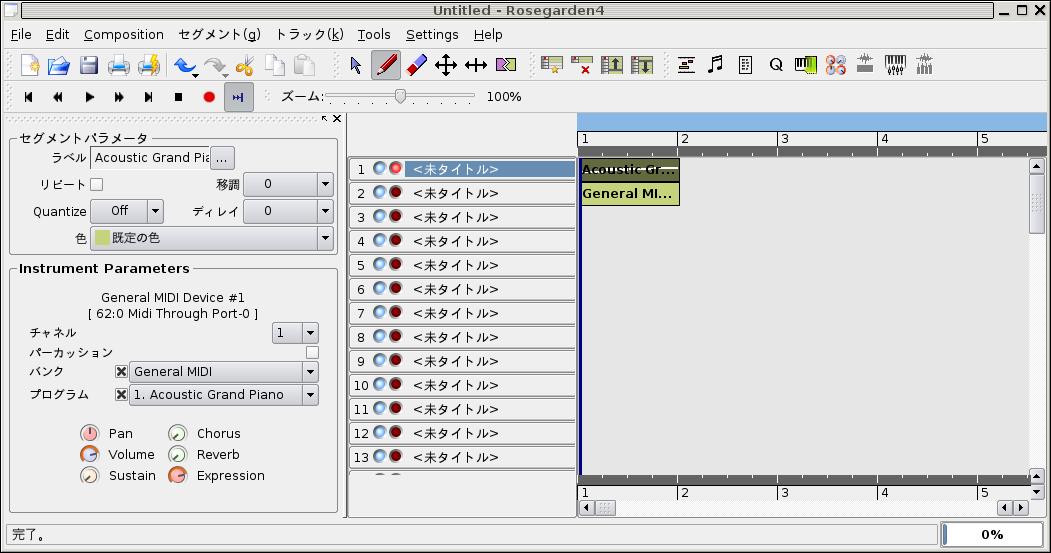
\includegraphics[width=10cm]{image200602/rosegarden4-1.png}
\end{frame}
\begin{frame}
 \frametitle{rosegarden4}
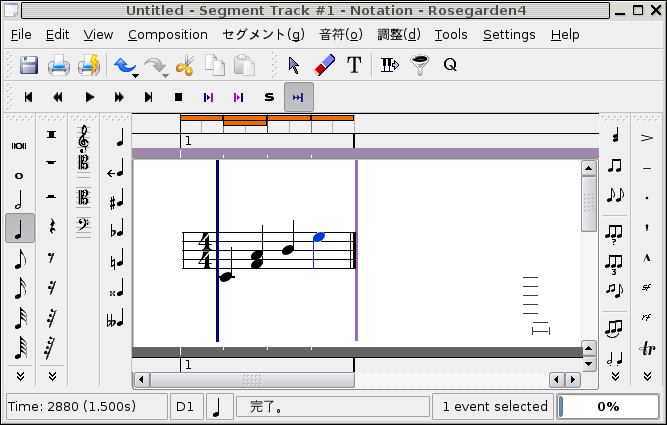
\includegraphics[width=10cm]{image200602/rosegarden4-2.png}
\end{frame}

\begin{frame}
 \frametitle{ardour}
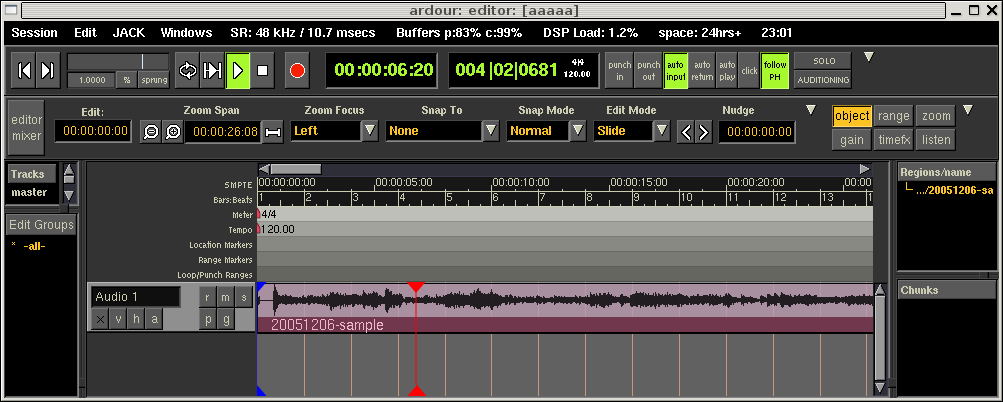
\includegraphics[width=10cm]{image200602/ardour2.png}
\end{frame}

\begin{frame}
 \frametitle{muse}
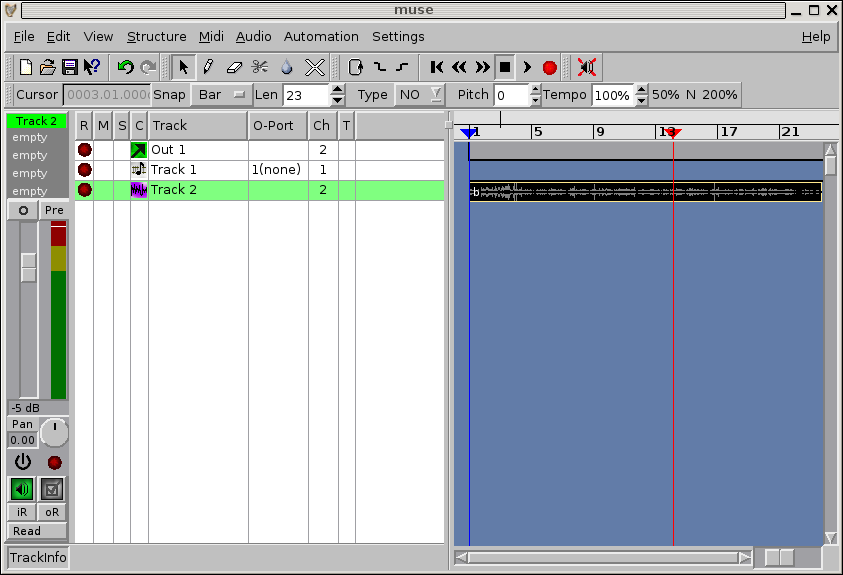
\includegraphics[width=10cm]{image200602/muse.png}
\end{frame}

 \subsection{そして今後は}
\begin{frame}
 \frametitle{行動計画}
\begin{itemize}
 \item debian-multimedia-policy: アプリの相互作業のための規格を整理。
 デフォルトでの動作を統一する。
 \item demudi-to-debian merge: パッケージをマージ。
       kernel-patch-realtime-lowlatency など
 \item LASH: それぞれのアプリを起動してから接続するまでの手間が面倒なのでその
       処理の自動化
 \item アプリ品質の改善。testsuiteを追加してregression suiteを構築すると
       ころからはじめる予定。
       そもそも使い方のわからないアプリケーションが多いので、棚卸しを最
       初の段階としては実施する。
\end{itemize}

\end{frame}

\end{document}
